%%%%%%%%%%%%%%%%%%%%%%%%%%%%% Define Article %%%%%%%%%%%%%%%%%%%%%%%%%%%%%%%%%%
\documentclass{article}
%%%%%%%%%%%%%%%%%%%%%%%%%%%%%%%%%%%%%%%%%%%%%%%%%%%%%%%%%%%%%%%%%%%%%%%%%%%%%%%

%%%%%%%%%%%%%%%%%%%%%%%%%%%%% Using Packages %%%%%%%%%%%%%%%%%%%%%%%%%%%%%%%%%%
\usepackage{geometry}

%Imgenes%
\usepackage{float} % Para usar [H]
\usepackage{graphicx}
%%%%%%%%%%%%%%%%%%
\usepackage{amssymb}
\usepackage{amsmath}
\usepackage{amsthm}
\usepackage{empheq}
\usepackage{mdframed}
\usepackage{booktabs}
\usepackage{lipsum}
\usepackage{graphicx}
\usepackage{color}
\usepackage{psfrag}
\usepackage{pgfplots}
\usepackage{bm}
%Para tablas%
\usepackage{array} % Para ajustar la alineación de columnas
\usepackage{booktabs} % Para mejorar la calidad de las líneas en la tabla


% Para Referencias
\usepackage[backend=biber, style=numeric]{biblatex}
\usepackage[colorlinks=true, linkcolor=blue, urlcolor=blue, citecolor=blue, filecolor=blue, bookmarks=true]{hyperref}
%%%%%%%%%%%%%%%%%%%%%%%%%%%%%%%%%%%%%%%%%%%%%%%%%%%%%%%%%%%%%%%%%%%%%%%%%%%%%%%

% Other Settings

%%%%%%%%%%%%%%%%%%%%%%%%%% Page Setting %%%%%%%%%%%%%%%%%%%%%%%%%%%%%%%%%%%%%%%
\geometry{a4paper}

%%%%%%%%%%%%%%%%%%%%%%%%%% Define some useful colors %%%%%%%%%%%%%%%%%%%%%%%%%%
\definecolor{ocre}{RGB}{243,102,25}
\definecolor{mygray}{RGB}{243,243,244}
\definecolor{deepGreen}{RGB}{26,111,0}
\definecolor{shallowGreen}{RGB}{235,255,255}
\definecolor{deepBlue}{RGB}{61,124,222}
\definecolor{shallowBlue}{RGB}{235,249,255}
%%%%%%%%%%%%%%%%%%%%%%%%%%%%%%%%%%%%%%%%%%%%%%%%%%%%%%%%%%%%%%%%%%%%%%%%%%%%%%%

%%%%%%%%%%%%%%%%%%%%%%%%%% Define an orangebox command %%%%%%%%%%%%%%%%%%%%%%%%
\newcommand\orangebox[1]{\fcolorbox{ocre}{mygray}{\hspace{1em}#1\hspace{1em}}}
%%%%%%%%%%%%%%%%%%%%%%%%%%%%%%%%%%%%%%%%%%%%%%%%%%%%%%%%%%%%%%%%%%%%%%%%%%%%%%%

%%%%%%%%%%%%%%%%%%%%%%%%%%%% English Environments %%%%%%%%%%%%%%%%%%%%%%%%%%%%%
\newtheoremstyle{mytheoremstyle}{3pt}{3pt}{\normalfont}{0cm}{\rmfamily\bfseries}{}{1em}{{\color{black}\thmname{#1}~\thmnumber{#2}}\thmnote{\,--\,#3}}
\newtheoremstyle{myproblemstyle}{3pt}{3pt}{\normalfont}{0cm}{\rmfamily\bfseries}{}{1em}{{\color{black}\thmname{#1}~\thmnumber{#2}}\thmnote{\,--\,#3}}
\theoremstyle{mytheoremstyle}
\newmdtheoremenv[linewidth=1pt,backgroundcolor=shallowGreen,linecolor=deepGreen,leftmargin=0pt,innerleftmargin=20pt,innerrightmargin=20pt,]{theorem}{Theorem}[section]
\theoremstyle{mytheoremstyle}
\newmdtheoremenv[linewidth=1pt,backgroundcolor=shallowBlue,linecolor=deepBlue,leftmargin=0pt,innerleftmargin=20pt,innerrightmargin=20pt,]{definition}{Definition}[section]
\theoremstyle{myproblemstyle}
\newmdtheoremenv[linecolor=black,leftmargin=0pt,innerleftmargin=10pt,innerrightmargin=10pt,]{problem}{Problem}[section]
%%%%%%%%%%%%%%%%%%%%%%%%%%%%%%%%%%%%%%%%%%%%%%%%%%%%%%%%%%%%%%%%%%%%%%%%%%%%%%%

%%%%%%%%%%%%%%%%%%%%%%%%%%%%%%% Plotting Settings %%%%%%%%%%%%%%%%%%%%%%%%%%%%%
\usepgfplotslibrary{colorbrewer}
\pgfplotsset{width=8cm,compat=1.9}
%%%%%%%%%%%%%%%%%%%%%%%%%%%%%%%%%%%%%%%%%%%%%%%%%%%%%%%%%%%%%%%%%%%%%%%%%%%%%%%

%%%%%%%%%%%%%%%%%%%%%%%%%%%%%%% Title & Author %%%%%%%%%%%%%%%%%%%%%%%%%%%%%%%%
\title{Use LATEX in Visual Studio Code}
\author{Diego Iván Perea Montealegre}
%%%%%%%%%%%%%%%%%%%%%%%%%%%%%%%%%%%%%%%%%%%%%%%%%%%%%%%%%%%%%%%%%%%%%%%%%%%%%%%

% Cargar el archivo de bibliografía
\addbibresource{bibliography.bib}

\begin{document}
    \maketitle
    Fist Step
   

    % Mostrar la lista
    % \textbf{MiKTeX}\footnote{MiKTeX is a distribution of LaTeX }
    \begin{itemize}
        \item Install \textcite{miktex} and  \textcite{strawberryperl}
        \item Open Visual Studio Code and install extension \texttt{LaTeX Workshop} from James Yu  and \texttt{LaTeX Snippets} from HaoyunQin
    \end{itemize}

    \begin{figure}[h]
        \centering
        
\includegraphics[width=0.7\textwidth ]{img/latexWorkshop.PNG}
        \caption{LaTeX Workshop}
        \label{fig:LaTeX Workshop}
    \end{figure}

    \begin{figure}[h]
        \centering
        
\includegraphics[width=0.7\textwidth,height=0.2\textwidth ]{img/latexSnippets.PNG}
        \caption{LaTeX Snippets}
        \label{fig:LaTeX Snippets}
    \end{figure}

    \maketitle
    Second Step
   

    % Mostrar la lista
    \begin{enumerate}
        \item Create a new folder
        \item In Settings, in search write "out dir"  and exactly in "Latex workshop - Latex:Out Dir" edit to '\%DIR\%/build'
        
        \begin{figure}[H]
            \centering
            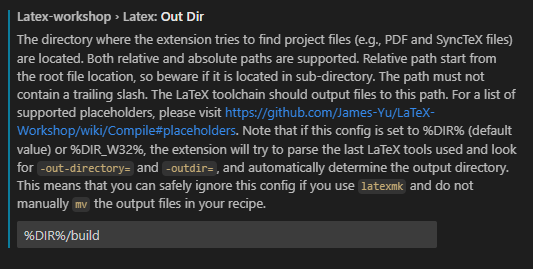
\includegraphics[width=0.7\textwidth ]{img/dirworshop.PNG}
            \caption{LaTeX build folder}
            \label{fig:LaTeX build folder}
        \end{figure}

        
        
        \item Create a new file with .tex
        \item play command and put the name of your file name 'pdflatex namefile.tex'
        
        \begin{figure}[h]
            \centering
            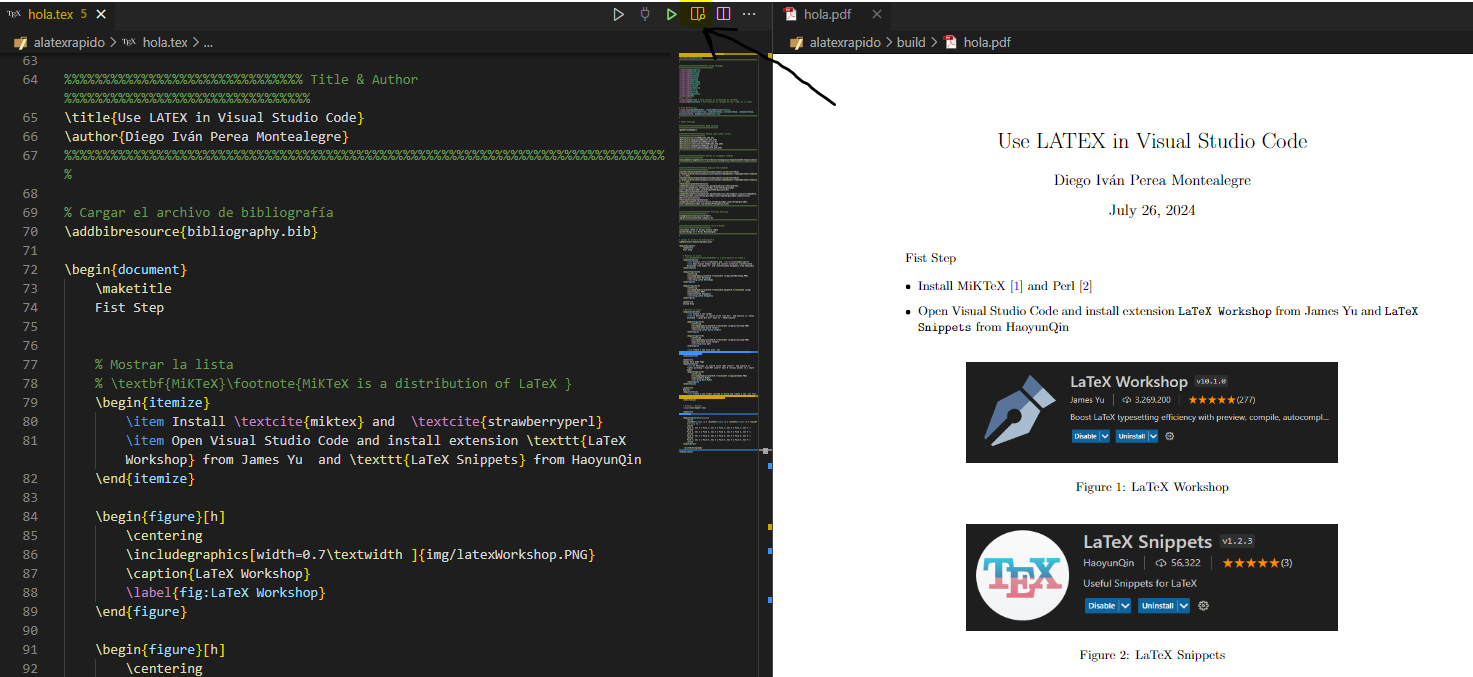
\includegraphics[width=1\textwidth]{img/viewpdf.PNG}
            \caption{View pdf click magnifying glass}
            \label{fig:View pdf click magnifying glass}
        \end{figure}
    \end{enumerate}
    
    \maketitle
    Change Dark mode Page
    \begin{itemize}
        \item In Settings, in search write "pdf invert"  and exactly in "Latex workshop - View-Pdf invert" edit 0 (normal white) to 1 (dark mode)
        \begin{figure}[h]
            \centering
            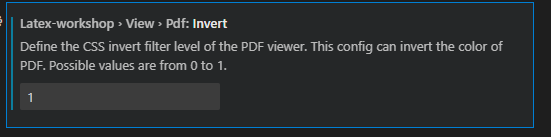
\includegraphics[width=0.7\textwidth ]{img/darkmode.PNG}
            \caption{Dark Mode}
            \label{fig:Dark Mode}
        \end{figure}
    \end{itemize}

    \maketitle
    Modules
    \begin{itemize}
        \item Create a new folder outside of build and create a new .tex file
        \item For put the module write \textbf{\texttt{\textbackslash input\{build/FolderCreatedTo/chapter.tex\}}}
    \end{itemize}

   
    % Modules / Modulos
    \maketitle
Bibliography
\begin{itemize}
    \item Create a new file with .bib
\end{itemize}
    
    \maketitle
    Tablas\\

    \begin{tabular}{|c|c|c|c|}
        \hline
        \textbf{Columna 1} & \textbf{Columna 2} & \textbf{Columna 3} & \textbf{Columna 4} \\
        \hline
        Fila 1, Col 1 & Fila 1, Col 2 & Fila 1, Col 3 & Fila 1, Col 4 \\
        \hline
        Fila 2, Col 1 & Fila 2, Col 2 & Fila 2, Col 3 & Fila 2, Col 4 \\
        \hline
        Fila 3, Col 1 & Fila 3, Col 2 & Fila 3, Col 3 & Fila 3, Col 4 \\
        \hline
        Fila 4, Col 1 & Fila 4, Col 2 & Fila 4, Col 3 & Fila 4, Col 4 \\
        \hline
    \end{tabular}

     \printbibliography

\end{document}